% Figure 4: hwloc Hardware Topology Hierarchy
% Standalone compilable: pdflatex fig4_hwloc_topology.tex
\documentclass[border=5pt]{standalone}
\usepackage{tikz}
\usetikzlibrary{shapes.geometric, arrows.meta, positioning, fit, backgrounds, calc, decorations.pathreplacing}

\begin{document}
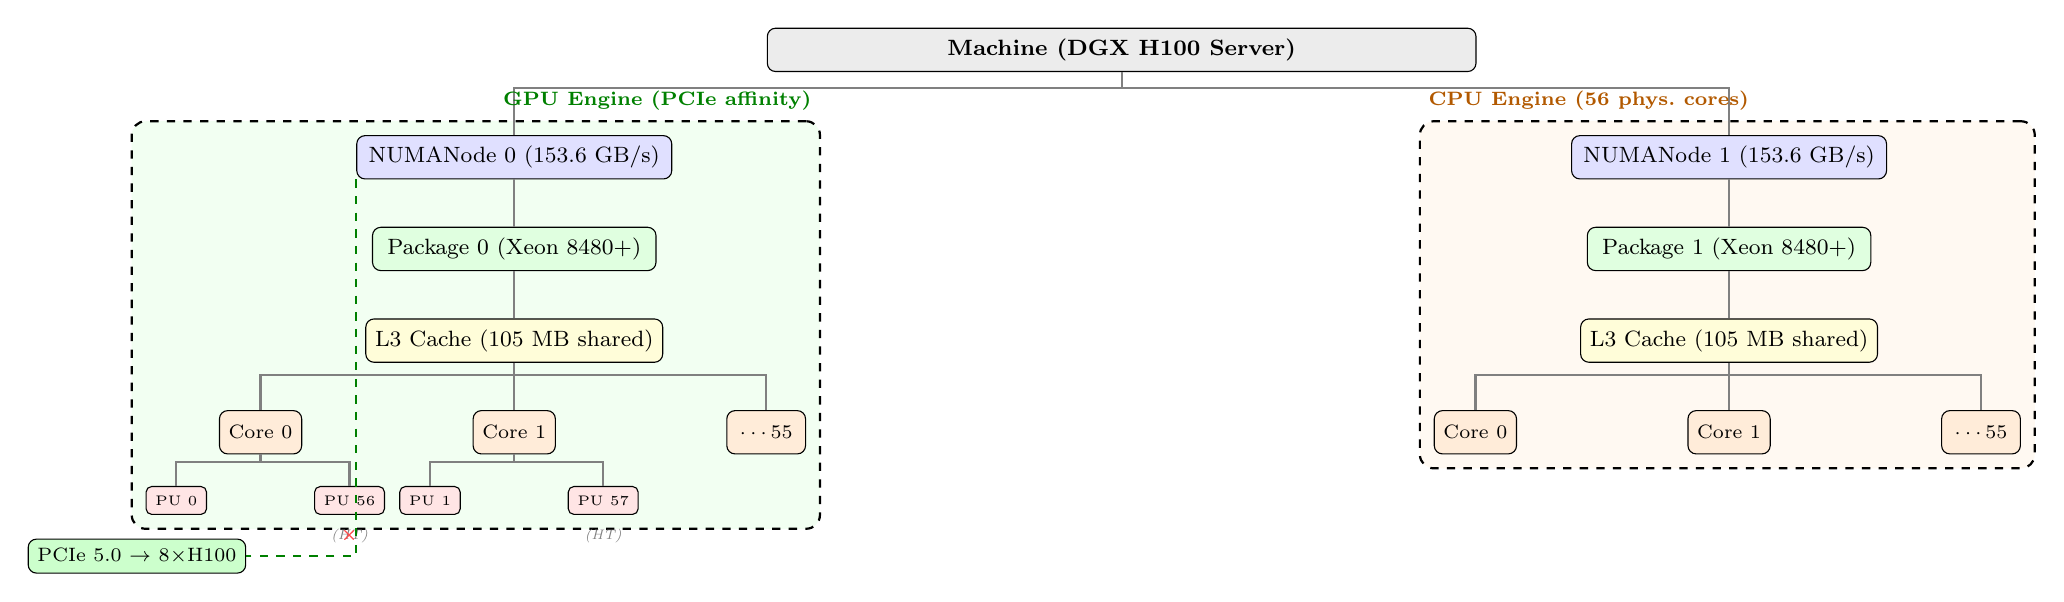
\begin{tikzpicture}[
    >=Stealth,
    node distance=0.5cm,
    level/.style={font=\footnotesize, draw, rounded corners=3pt, minimum height=0.55cm, align=center},
    machine/.style={level, fill=gray!15, minimum width=9cm, font=\footnotesize\bfseries},
    numa/.style={level, fill=blue!12, minimum width=4.0cm},
    pkg/.style={level, fill=green!12, minimum width=3.6cm},
    l3/.style={level, fill=yellow!15, minimum width=3.2cm},
    core/.style={level, fill=orange!15, minimum width=1.0cm, font=\scriptsize},
    pu/.style={draw, fill=red!10, rounded corners=2pt, minimum width=0.6cm, minimum height=0.35cm, font=\tiny, align=center},
    engine/.style={draw, thick, dashed, rounded corners=5pt, inner sep=5pt},
    elabel/.style={font=\scriptsize\bfseries},
    arrow/.style={-, thick, gray},
    brace/.style={decorate, decoration={brace, amplitude=5pt, raise=2pt}},
  ]

  % --- Machine ---
  \node[machine] (machine) {Machine (DGX H100 Server)};

  % --- NUMA Nodes ---
  \node[numa, below left=0.8cm and 1.2cm of machine] (numa0) {NUMANode 0 (153.6 GB/s)};
  \node[numa, below right=0.8cm and 1.2cm of machine] (numa1) {NUMANode 1 (153.6 GB/s)};

  \draw[arrow] (machine.south) -- ++(0,-0.2) -| (numa0.north);
  \draw[arrow] (machine.south) -- ++(0,-0.2) -| (numa1.north);

  % --- Packages ---
  \node[pkg, below=0.6cm of numa0] (pkg0) {Package 0 (Xeon 8480+)};
  \node[pkg, below=0.6cm of numa1] (pkg1) {Package 1 (Xeon 8480+)};

  \draw[arrow] (numa0) -- (pkg0);
  \draw[arrow] (numa1) -- (pkg1);

  % --- L3 Cache ---
  \node[l3, below=0.6cm of pkg0] (l3_0) {L3 Cache (105 MB shared)};
  \node[l3, below=0.6cm of pkg1] (l3_1) {L3 Cache (105 MB shared)};

  \draw[arrow] (pkg0) -- (l3_0);
  \draw[arrow] (pkg1) -- (l3_1);

  % --- Cores (Socket 0) ---
  \node[core, below left=0.6cm and 0.8cm of l3_0] (c0) {Core 0};
  \node[core, below=0.6cm of l3_0] (c1) {Core 1};
  \node[core, below right=0.6cm and 0.8cm of l3_0] (cdots0) {$\cdots$\,55};

  \draw[arrow] (l3_0.south) -- ++(0,-0.15) -| (c0.north);
  \draw[arrow] (l3_0.south) -- (c1.north);
  \draw[arrow] (l3_0.south) -- ++(0,-0.15) -| (cdots0.north);

  % --- PUs (Socket 0, Core 0) ---
  \node[pu, below left=0.4cm and 0.15cm of c0] (pu0) {PU 0};
  \node[pu, below right=0.4cm and 0.15cm of c0] (pu56) {PU 56};

  \draw[arrow] (c0.south) -- ++(0,-0.1) -| (pu0.north);
  \draw[arrow] (c0.south) -- ++(0,-0.1) -| (pu56.north);

  % --- PUs (Socket 0, Core 1) ---
  \node[pu, below left=0.4cm and 0.15cm of c1] (pu1) {PU 1};
  \node[pu, below right=0.4cm and 0.15cm of c1] (pu57) {PU 57};

  \draw[arrow] (c1.south) -- ++(0,-0.1) -| (pu1.north);
  \draw[arrow] (c1.south) -- ++(0,-0.1) -| (pu57.north);

  % --- Cores (Socket 1) ---
  \node[core, below left=0.6cm and 0.8cm of l3_1] (c56) {Core 0};
  \node[core, below=0.6cm of l3_1] (c57) {Core 1};
  \node[core, below right=0.6cm and 0.8cm of l3_1] (cdots1) {$\cdots$\,55};

  \draw[arrow] (l3_1.south) -- ++(0,-0.15) -| (c56.north);
  \draw[arrow] (l3_1.south) -- (c57.north);
  \draw[arrow] (l3_1.south) -- ++(0,-0.15) -| (cdots1.north);

  % --- PU labels ---
  \node[font=\tiny\itshape, text=gray, below=0.05cm of pu56] {(HT)};
  \node[font=\tiny\itshape, text=gray, below=0.05cm of pu57] {(HT)};

  % --- Engine assignments ---
  \begin{scope}[on background layer]
    \node[engine, fill=green!5, fit=(numa0)(pkg0)(l3_0)(c0)(c1)(cdots0)(pu0)(pu56)(pu1)(pu57)] (gpu_zone) {};
    \node[engine, fill=orange!5, fit=(numa1)(pkg1)(l3_1)(c56)(c57)(cdots1)] (cpu_zone) {};
  \end{scope}

  \node[elabel, color=green!50!black, anchor=south east] at (gpu_zone.north east) {GPU Engine (PCIe affinity)};
  \node[elabel, color=orange!70!black, anchor=south west] at (cpu_zone.north west) {CPU Engine (56 phys.\ cores)};

  % --- PCIe annotation ---
  \node[draw, fill=green!20, rounded corners=3pt, font=\scriptsize, below=0.3cm of pu0, xshift=-0.5cm] (pcie) {PCIe 5.0 $\to$ 8$\times$H100};
  \draw[arrow, green!50!black, dashed] (numa0.south west) |- (pcie.east);

  % --- Use / Skip annotations ---
  \node[font=\tiny\bfseries, color=green!50!black, anchor=north] at ([yshift=-0.05cm]pu0.south) {\checkmark};
  \node[font=\tiny\bfseries, color=red!70, anchor=north] at ([yshift=-0.05cm]pu56.south) {\texttimes};

\end{tikzpicture}
\end{document}
